\section{Ice dynamics, the PISM view}\label{sec:dynamics}

\subsection{Two stress balance models: SIA and SSA}\index{PISM!SIA}\index{PISM!SSA}  At each time-step of a typical PISM run, the geometry, temperature, and basal strength of the ice sheet are included into stress (momentum) balance equations to determine the velocity of the flowing ice.   The ``full'' stress balance equations for flowing ice form a non-Newtonian Stokes model \cite{Fowler}.  PISM does not attempt to solve the Stokes equations themselves, however.  Instead it can numerically solve, in parallel, two different shallow approximations which are well-suited to ice sheet and ice shelf systems:
\begin{itemize}
\item the non-sliding shallow ice approximation (SIA)\index{SIA (shallow ice approximation)} \cite{Hutter}, also called the ``lubrication approximation'' \cite{Fowler}, which describes ice as flowing by shear in planes parallel to the geoid, with a strong connection of the ice base to the bedrock, and
\item the shallow shelf approximation (SSA)\index{SSA (shallow shelf approximation)} \cite{WeisGreveHutter}, which describes a membrane-type flow of floating ice \cite{Morland}, or of grounded ice which is sliding over a weak base \cite{MacAyeal,SchoofStream}.
\end{itemize}

The SIA\index{SIA (shallow ice approximation)!applicability} equations are easier to solve numerically than the SSA, and easier to parallelize, because they are local in each column of ice.\index{parallelization!relative ease of, between SIA and SSA}  Specifically, they describe the vertical shear stress as a local function of the driving stress \cite{Paterson}.  They can confidently be applied to those grounded parts of ice sheets for which the basal ice is frozen to the bedrock, or which is minimally sliding, and where the bed topography is relatively slowly-varying in the map-plane \cite{Fowler}.  These characteristics apply to the majority (by area) of the Greenland and Antarctic ice sheets.

We solve the SIA with a non-sliding base because the traditional \cite{Greve,HuybrechtsdeWolde,PayneBaldwin} addition of ad~hoc ``sliding laws''\index{SIA (shallow ice approximation)!sliding laws} into the SIA stress balance, and especially schemes which ``switch on'' at the pressure-melting temperature \cite{EISMINT00}, have bad continuum  \cite{Fowler01} and numerical \cite[appendix B]{BBssasliding} modeling consequences.

The SSA\index{SSA (shallow shelf approximation)!applicability} equations can confidently be applied to large floating ice shelves, which have small depth-to-width ratio and negligible basal resistance \cite{Morland,MorlandZainuddin}.  The flow speeds in ice shelves are frequently an order-of-magnitude higher than in the non-sliding, grounded parts of ice sheets.

Terrestrial ice sheets also have fast-flowing grounded parts, however, called ``ice streams'' or ``outlet glaciers'' \cite{TrufferEchelmeyer}.  Such features appear at the margin of, and sometimes well into the interior of, the Greenland \cite{Joughinetal2001}\index{Ice Sheets!Greenland ice sheet} and Antarctic \cite{BamberVaughanJoughin}\index{Ice Sheets!Antarctic ice sheet} ice sheets.  Describing these faster-flowing grounded parts of ice sheets requires something more than the non-sliding SIA.  This is because adjacent columns of ice which have different amounts of basal resistance exert strong ``longitudinal'' or ``membrane'' stresses \cite{SchoofStream} on each other.

In PISM the SSA may be used as a ``sliding law'' for grounded ice which is already modeled everywhere by the non-sliding SIA \cite{BBssasliding,Winkelmannetal2011}.  For grounded ice, in addition to including shear in planes parallel to the geoid, we must balance the membrane stresses where there is sliding.  This inclusion of a membrane stress balance is especially important when there are spatial and/or temporal changes in basal strength.  This ``sliding law'' role for the SSA is in addition to its more obvious role in ice shelf modeling.  The SSA plays both roles in a PISM whole ice sheet model in which there are large floating ice shelves (e.g.~as in Antarctica \cite{Golledgeetal2012ant,Martinetal2011,Winkelmannetal2011}; see also section \ref{sec:ross} of the current Manual).

The ``SIA+SSA hybrid'' model is recommended for most whole ice sheet modeling purposes because it seems to be a good compromise given currently-available data and computational power.  A related hybrid model described by Pollard and deConto \cite{PollardDeConto} adds the shear to the SSA solution in a slightly-different manner, but it confirms the success of the hybrid concept.

By default, however, PISM does not turn on (activate) the SSA solver.  This is because a decision to solve the SSA must go with a conscious user choice about basal strength.  The user must both use a command-line option to turn on the SSA (e.g. option \texttt{-stress_balance ssa}; see section \ref{subsect:stressbalance}) and also make choices in input files and runtime options about basal strength (see section \ref{subsect:basestrength}).  Indeed, uncertainties in basal strength boundary conditions usually dominate the modeling error made by not including higher-order stresses in the balance.  

When the SSA model is applied a parameterized sliding relation must be chosen.  A well-known SSA model with a linear basal resistance relation is the Siple Coast (Antarctica) ice stream model by MacAyeal \cite{MacAyeal}.  The linear sliding law choice is explained by supposing the saturated till is a linearly-viscous fluid.  A free boundary problem with the same SSA balance equations but a different sliding law is the Schoof \cite{SchoofStream} model of ice streams, using a plastic (Coulomb) sliding relation.  In this model ice streams appear where there is ``till failure'' \cite{Paterson}, i.e.~where the basal shear stress exceeds the yield stress.  In this model the location of ice streams is not imposed in advance.

As noted, both the SIA and SSA models are \emph{shallow} approximations.  These equations are derived from the Stokes equations by distinct small-parameter arguments, both based on a small depth-to-width ratio for the ice sheet.  For the small-parameter argument in the SIA case see \cite{Fowler}.  For the corresponding SSA argument, see \cite{WeisGreveHutter} or the appendices of \cite{SchoofStream}.  Schoof and Hindmarsh \cite{SchoofHindmarsh} have analyzed the connections between these shallowest models and higher-order models, while \cite{GreveBlatter2009} discusses ice dynamics and stress balances comprehensively.  Note that SIA, SSA, and higher-order models all approximate the pressure as hydrostatic.

Instead of a SIA+SSA hybrid model as in PISM, one might use the Stokes equations, or a ``higher-order'' model (i.e.~less-shallow approximations \cite{Blatter,Pattyn03}), but this immediately leads to a resolution-versus-stress-inclusion tradeoff.  The amount of computation per map-plane grid location is much higher in higher-order models, although careful numerical analysis can generate large performance improvements for such equations \cite{BrownSmithAhmadia2013}.

Time-stepping solutions of the mass conservation and energy conservation equations, which use the ice velocity for advection, can use any of the SIA or SSA or SIA+SSA hybrid stress balances.  No user action is required to turn on these conservation models.  They can be turned off by user options \texttt{-no_mass} (ice geometry does not evolve) or \texttt{-energy none} (ice enthalpy and temperature does not evolve), respectively.

\newenvironment{tightlist}{\begin{itemize}  \vspace{-0.15in}\addtolength{\itemsep}{-0.5\baselineskip} } {\vspace{-0.1in} \end{itemize}}

\newcommand{\nolist}[1]{[\emph{#1}] \vspace{0.1in}}

\begin{table}[ht]
\small\medskip
\begin{tabular}{p{0.22\linewidth}p{0.40\linewidth}p{0.32\linewidth}}
\toprule
\textbf{Model} & \textbf{Assumptions} & \textbf{Required data} \\
\midrule
\vspace{2mm}  \emph{perfectly-plastic ice} \small & \vspace{2mm}\emph{steady state}; ice has shear stresses below a pre-determined ice ``yield stress''; also needs pre-determined location of ice sheet margin  \vspace{2mm} & \vspace{2mm} \begin{tightlist} \item bed elevation \end{tightlist} \\
\emph{balance velocities} \small & \emph{steady state}; ice flows down surface gradient \cite{JoughinetalGrBal97} & \nolist{same as above, plus:}  \begin{tightlist} \item surface mass balance \item (initial) ice thickness \end{tightlist} \\
\textsc{isothermal SIA} & non-sliding lubrication flow, fixed softness \cite{BLKCB,EISMINT96} & \nolist{same as above, but time-dependence is allowed} \\
\textsc{thermo-coupled SIA} & non-sliding lubrication flow, temperature-dependent softness \cite{BBL,EISMINT00} & \nolist{same as above, plus:} \begin{tightlist} \item surface temperature \item geothermal flux \end{tightlist} \\
\textsc{polythermal SIA} & allows liquid water fraction in temperate ice; conserves energy better \cite{AschwandenBuelerKhroulevBlatter,Greve} \vspace{2mm} & \nolist{same as above} \\
\textsc{SIA + SSA hybrid} & SSA as a sliding law for thermo-coupled SIA \cite{BBssasliding,Winkelmannetal2011}; polythermal by default & \nolist{same as above, plus:} \begin{tightlist} \item model for subglacial water \item model for basal resistance \end{tightlist} \\
\emph{Blatter-Pattyn} \small & ``higher-order'', bridging stresses \cite{Blatter,Pattyn03,SchoofCoulombBlatter} & \nolist{same as above} \\
\bottomrule
\end{tabular}
\normalsize
\caption{Hierarchy of flow models in PISM for the grounded
  parts of ice sheets.  Listed from most to fewest simplifying assumptions \emph{and}
  from least to greatest need for boundary data.  The \emph{italicized} models
  are planned for future versions of PISM but are not implemented so far.}
\label{tab:modelhierarchy}
\end{table}


\subsection{A hierarchy of simplifying assumptions for grounded ice flow}
\label{sec:model-hierarchy}\index{PISM!hierarchy of simplifying assumptions}
Table \ref{tab:modelhierarchy} describes a hierarchy of models, listed roughly in order of increasing effectiveness in modeling grounded ice sheets with fast flow features.  This is also the order of increasing need for data to serve as boundary and initial conditions, however, as also described in the Table.

\begin{figure}[ht]
  \centering
  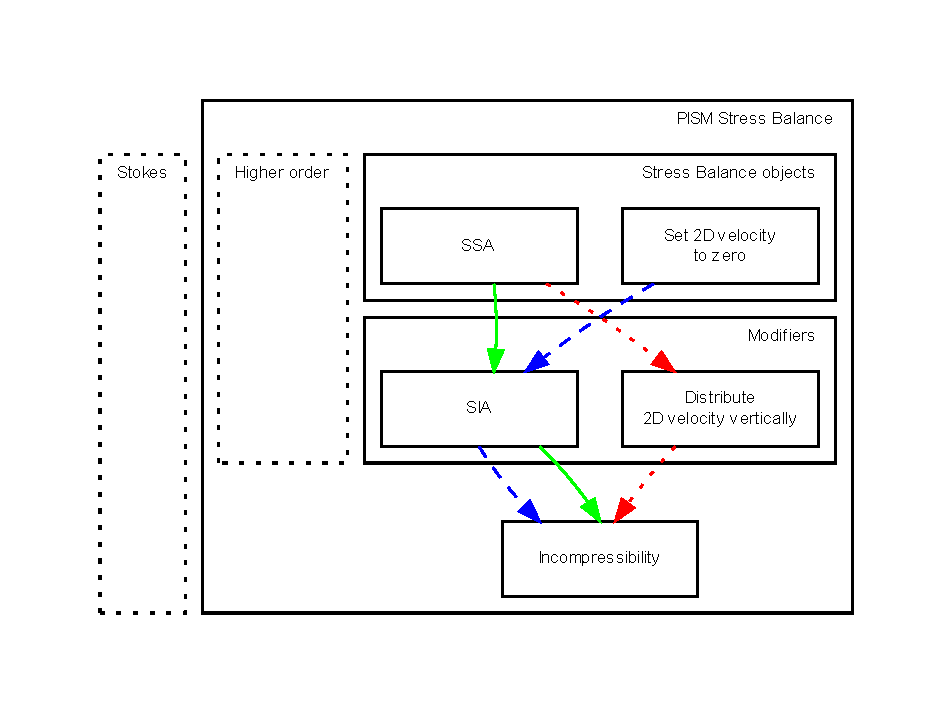
\includegraphics[width=6in]{stressbalance}
  \caption{The SIA-only, SSA-only, and SIA+SSA hybrid models represent different ``routes'' through stress balance PISM components.  In each case the inputs are ice geometry and boundary stresses, and the final output is a three-dimensional velocity field within the ice.}
  \label{fig:stressbalance}
\end{figure}

It may also be helpful to view the implemented stress balances as PISM software components (C++ classes).  Figure \ref{fig:stressbalance} shows the sequences of actions taken by the SIA-only, SSA-only, and SIA+SSA hybrid model components.  In each case a membrane stress solution is generated first, then a distribution of vertical shear in the column of ice is generated second, and finally a use of incompressibility computes the vertical component of the velocity.  The nonsliding SIA-only model has a trivialized membrane stress solution.  The SSA-only model has a trivialized computation of vertical shear.


\subsection{Evolutionary versus diagnostic modeling} \label{subsect:basicmodes}\index{PISM!evolution run}\index{PISM!diagnostic run}    The main goal of a numerical ice sheet model like PISM is to be a dynamical system which evolves as similarly as possible to the modeled ice sheet.  Such a goal assumes one has the ``right'' climate inputs and parameter choices at each time step.  It also assumes one has the ``right'' initial conditions, such as an adequate description of the present state of the ice sheet, but this assumption is rarely satisfied.  Instead a variety of heuristics must be used to minimally-initialize an ice sheet model.  For options associated to establishing mathematical initial conditions when first starting PISM, see section \ref{sec:initboot}.

Inside PISM are evolution-in-time partial differential equations which are solved by taking small time steps.  ``Small'' may vary from thousandths to tens of model years, in practice, depending primarily on grid resolution, but also on modeled ice geometry and flow speed.  Time steps are chosen adaptively in PISM, according to the stability criteria of the combined numerical methods \cite{BBssasliding,BBL}.

However, especially for ice streams and shelves, non-time-stepping ``diagnostic'' solution of the stress balance partial differential equations might be the desired computation, and PISM can also produce such ``diagnostic'' velocity fields.  Such computations necessarily assume that the ice geometry, viscosity, and boundary stresses are known.  Because of the slowness of the ice, in the sense that inertia can be neglected in the stress balance \cite{Fowler}, such computations can determine the ice velocity.

Sections \ref{sec:start} and \ref{sec:ross} give examples illustrating evolutionary and diagnostic modes of PISM, respectively.  The first describes time-stepping evolution models for the Greenland ice sheet, while the second describes a diagnostic SSA model for the Ross ice shelf.


\subsection{Climate inputs, and their interface with ice dynamics}
\label{sec:climate-inputs}  

\begin{figure}[ht]
  \centering
  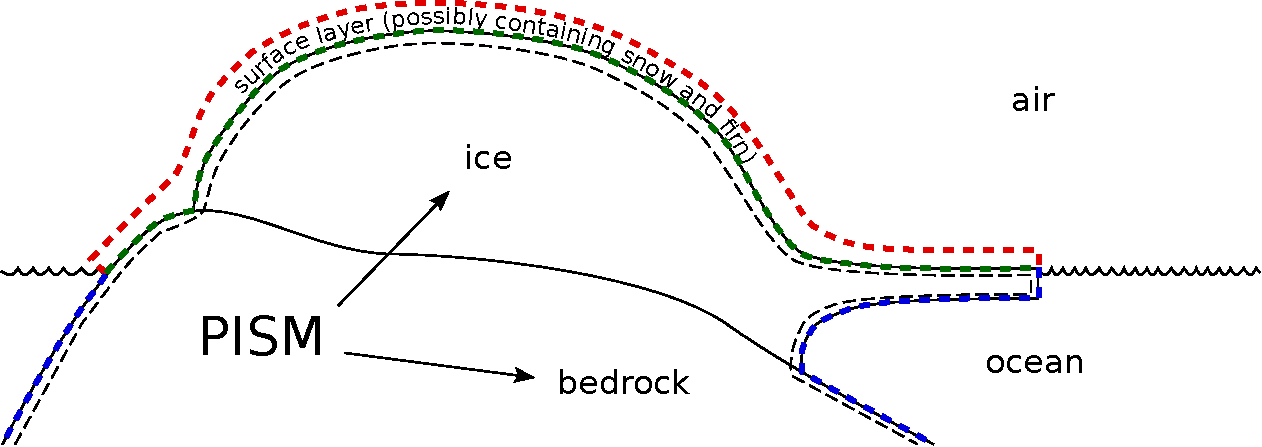
\includegraphics[width=6in]{figs/climate-cartoon.pdf}
  \caption{PISM's view of interfaces between an ice sheet and the outside world}
  \label{fig:climate-inputs}
\end{figure}

Because PISM's job is to approximate ice flow, its ``world view'' is centered around ice dynamics.  The discussion of boundary conditions in this Manual is thus ice-dynamics-centric.  On the other hand, there is no constraint on the nature of, or completeness of, climate models which could be coupled to PISM.  This section therefore explains a PISM organizing principle, namely that \emph{climate inputs affect ice dynamics by a well-defined interface}.

Almost no attempt is made here to describe the physics of the climate around ice sheets, so see \cite{massbalanceglossary} for terminology and \cite{Hock05} for a review of how surface melt can be modeled.  See the Climate Forcing Manual for much more information on PISM's climate-coupling-related options and on the particular fields which are shared between the ice dynamics core and the climate model.  Table \ref{tab:ice-dynamics-bc} lists fields which are needed as boundary conditions at the interfaces.

All PISM ice sheet models have some kind of interface (\textcolor{ForestGreen}{\textbf{green}} in Figure \ref{fig:climate-inputs}) to a subaerial surface processes layer containing snow, firn, and liquid (or refrozen) runoff.  The surface layer is assumed to cover the whole surface of the ice, and all grounded areas that the ice might occupy, including ablation areas and ice-free land.  We also always have an interface (\textcolor{blue}{\textbf{blue}}) to the ocean, but this interface is inactive if there is no floating ice.

\begin{table}[ht]
  \centering
 \begin{tabular}{p{0.45\linewidth}p{0.5\linewidth}}
    \toprule
    \textbf{Boundary surface} & \textbf{Fields (conditions)} \\
    \midrule
    upper surface of the surface processes layer (\textcolor{red}{\textbf{red}}) & \emph{optional}; typically: air temperature, precipitation \\
    top ice surface, but below firn (\textcolor{ForestGreen}{\textbf{green}}) & \emph{required}: boundary temperature (or enthalpy), mass flux (SMB) into the ice\\
    ice shelf basal surface (\textcolor{blue}{\textbf{blue}}) & \emph{required}: mass flux into the ocean, boundary temperature\\
    bottom surface of thermally-modeled bedrock layer (not shown) & \emph{required}: geothermal flux\\
   \bottomrule
  \end{tabular}
\caption{Boundary conditions required by PISM's ice dynamics core; see Figure \ref{fig:climate-inputs}.  The optional \textcolor{red}{\textbf{red}} interface is absent if PISM does not ``own'' the surface processes layer.}
\label{tab:ice-dynamics-bc}
\end{table}

The surface processes layer might be very simple.  It might either read the important fields from a file or otherwise transfer them from a separate (non-PISM) climate model.  If, however, the surface processes layer is ``owned'' by the PISM model then there is an additional interface (\textcolor{red}{\textbf{red}}) to the atmosphere above.  In no case does PISM ``own'' the atmosphere; if it has an interface to the atmosphere at all then it reads atmosphere fields from a file or otherwise transfers them from a climate model.

Regarding the base of the ice, the temperature of a layer of bedrock in contact with grounded ice is generally included in PISM's conservation of energy model; see subsections \ref{subsect:coords} and \ref{subsect:grid}.   Also, as described in section \ref{subsect:beddef}, PISM can apply an optional bed deformation component approximating the movement of the Earth's crust and upper mantle in response to changing ice load.  In these senses everything below the black dashed line in Figure \ref{fig:climate-inputs} is always ``owned'' by PISM.

The PISM ice dynamics core would like to get the required fields listed in Table
\ref{tab:ice-dynamics-bc} directly from observations or measurements, or directly from a GCM.  In many realistic modeling situations, however, PISM code must be used for all or part of the surface processes modeling necessary to provide the ice-dynamics core with the needed fields.  Due to differences in model resolutions and required down-scaling, this need for some PISM-based boundary-processes modelling may occur even in some cases where PISM is coupled to a GCM.  Thus, to be able to use the data that is available, a PISM run might use components that are responsible for modeling surface (snow) processes or sub-shelf/ocean interaction.  These components might be very minimal, merely turning data that we already have into data in the right units and with the right metadata.

\begin{figure}[ht]
  \centering
  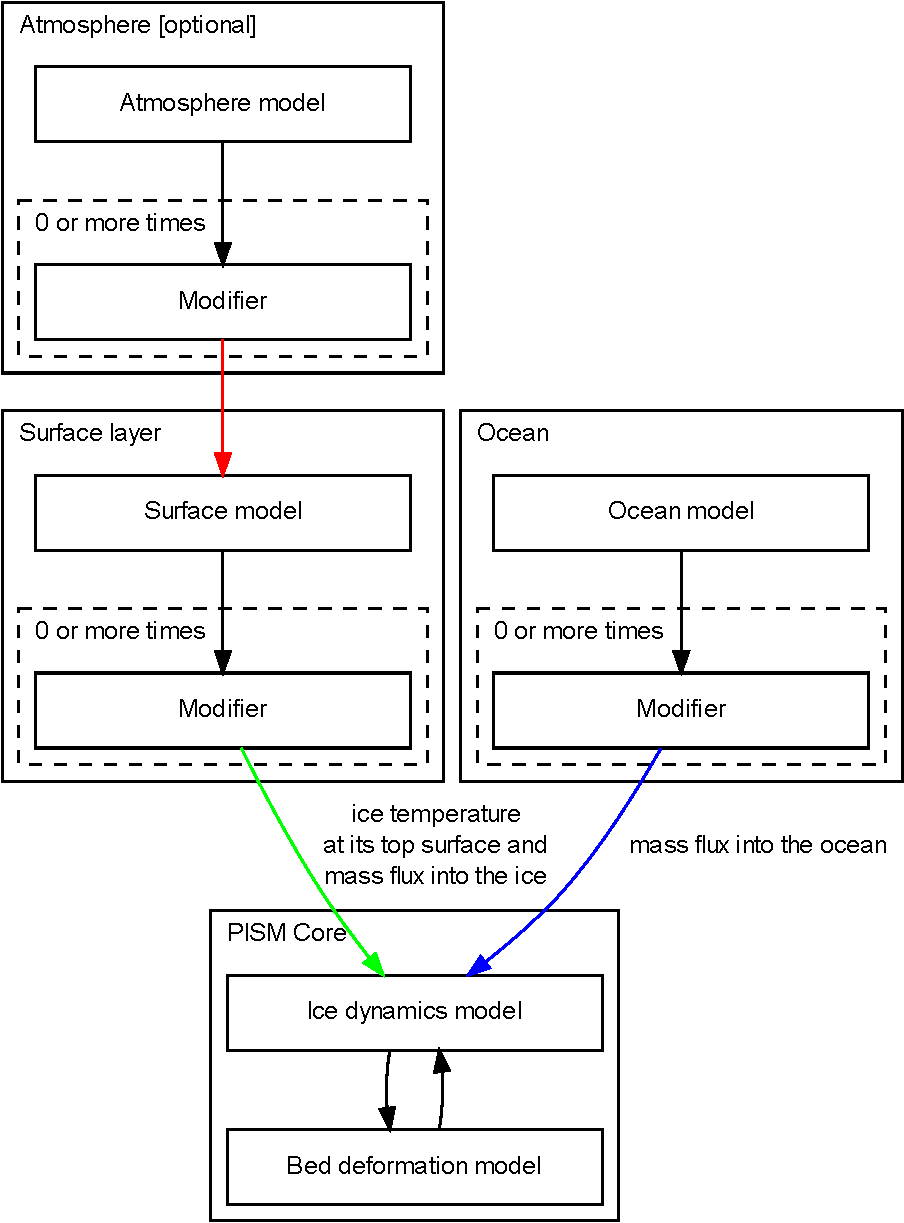
\includegraphics[width=4.0in]{figs/data-flow.pdf}
  \caption{PISM climate input data flow. Colored arrows correspond to interfaces in
    Figure \ref{fig:climate-inputs}.}
  \label{fig:climate-input-data-flow}
\end{figure}

Thus we have PISM's design: the ice-dynamics PISM core does not contain any parameterization or other model for boundary mass or energy fluxes into or out of the ice.  These boundary parameterizations and models are present in the PISM source code, however, as instances of \emph{PISMComponent} classes.  This simplifies customizing and debugging PISM's climate inputs, and it promotes code reuse.  It isolates the code that needs to be changed to couple PISM to different climate models.

The classes \mbox{\emph{PISMSurfaceModel}}, \mbox{\emph{PISMAtmosphereModel}}, and \mbox{\emph{PISMOceanModel}} are all derived from \mbox{\emph{PISMComponent}}.  Corresponding to the \textcolor{red}{\textbf{red}} dashed line in Figure~\ref{fig:climate-inputs}, a \mbox{\emph{PISMAtmosphereModel}} might not even be present in some PISM configurations.  While they are required, \emph{PISMSurfaceModel} and \emph{PISMOceanModel} may contain (hide) anything from nearly-trivial parameterizations of ice surface temperatures and mass fluxes to a GCM of great complexity.  

The ``modifiers'' in Figure \ref{fig:climate-input-data-flow} adjust the
climate model inputs.  Modifiers can be chained together so that multiple modifications
are made to the outputs of the original component.  For example,
ice-core-derived air temperature offsets, used to model the space-time
distribution of paleo-climatic surface temperature, is an example of an
implemented modifier.  Please see the Climate Forcing Manual for
a list of climate components and modifiers included in PISM source code and other details.
Users wishing to customize PISM's climate inputs and/or couple PISM to a climate
model should additionally see the \emph{PISM Source Browser} at \url{\PISMBROWSERURL}
and the documentation therein.

Figure~\ref{fig:climate-input-data-flow} illustrates the data flow needed
by the ice dynamics core.  The data flow in the other direction, i.e.~needed by the
model to which PISM is coupled, depends on particular modeling choices, but
great flexibility is allowed.

Why describe all this structure here?  On the one hand, some users may be interested
in coupling PISM to other models.  On the other hand, the PISM authors do not
claim expertise in modeling atmosphere, ocean, or even snow processes.  This
separation has a definite code-reliability purpose.  PISM users
are ultimately responsible for providing the climate inputs they intend.
